\section{add_biguint}
\label{add_biguint}

Take uint128 as example, the same as other texs.

\begin{enumerate}
    \item target
        implenment the addition of two biguints.
    \item constraints_logic
        \begin{itemize}
            \item equation for gate
            \item sumcheck between ouptput and limbs
            \item rangecheck for limbs
        \end{itemize}
    \item circuit layout
        \begin{figure}[!ht]
            \centering
            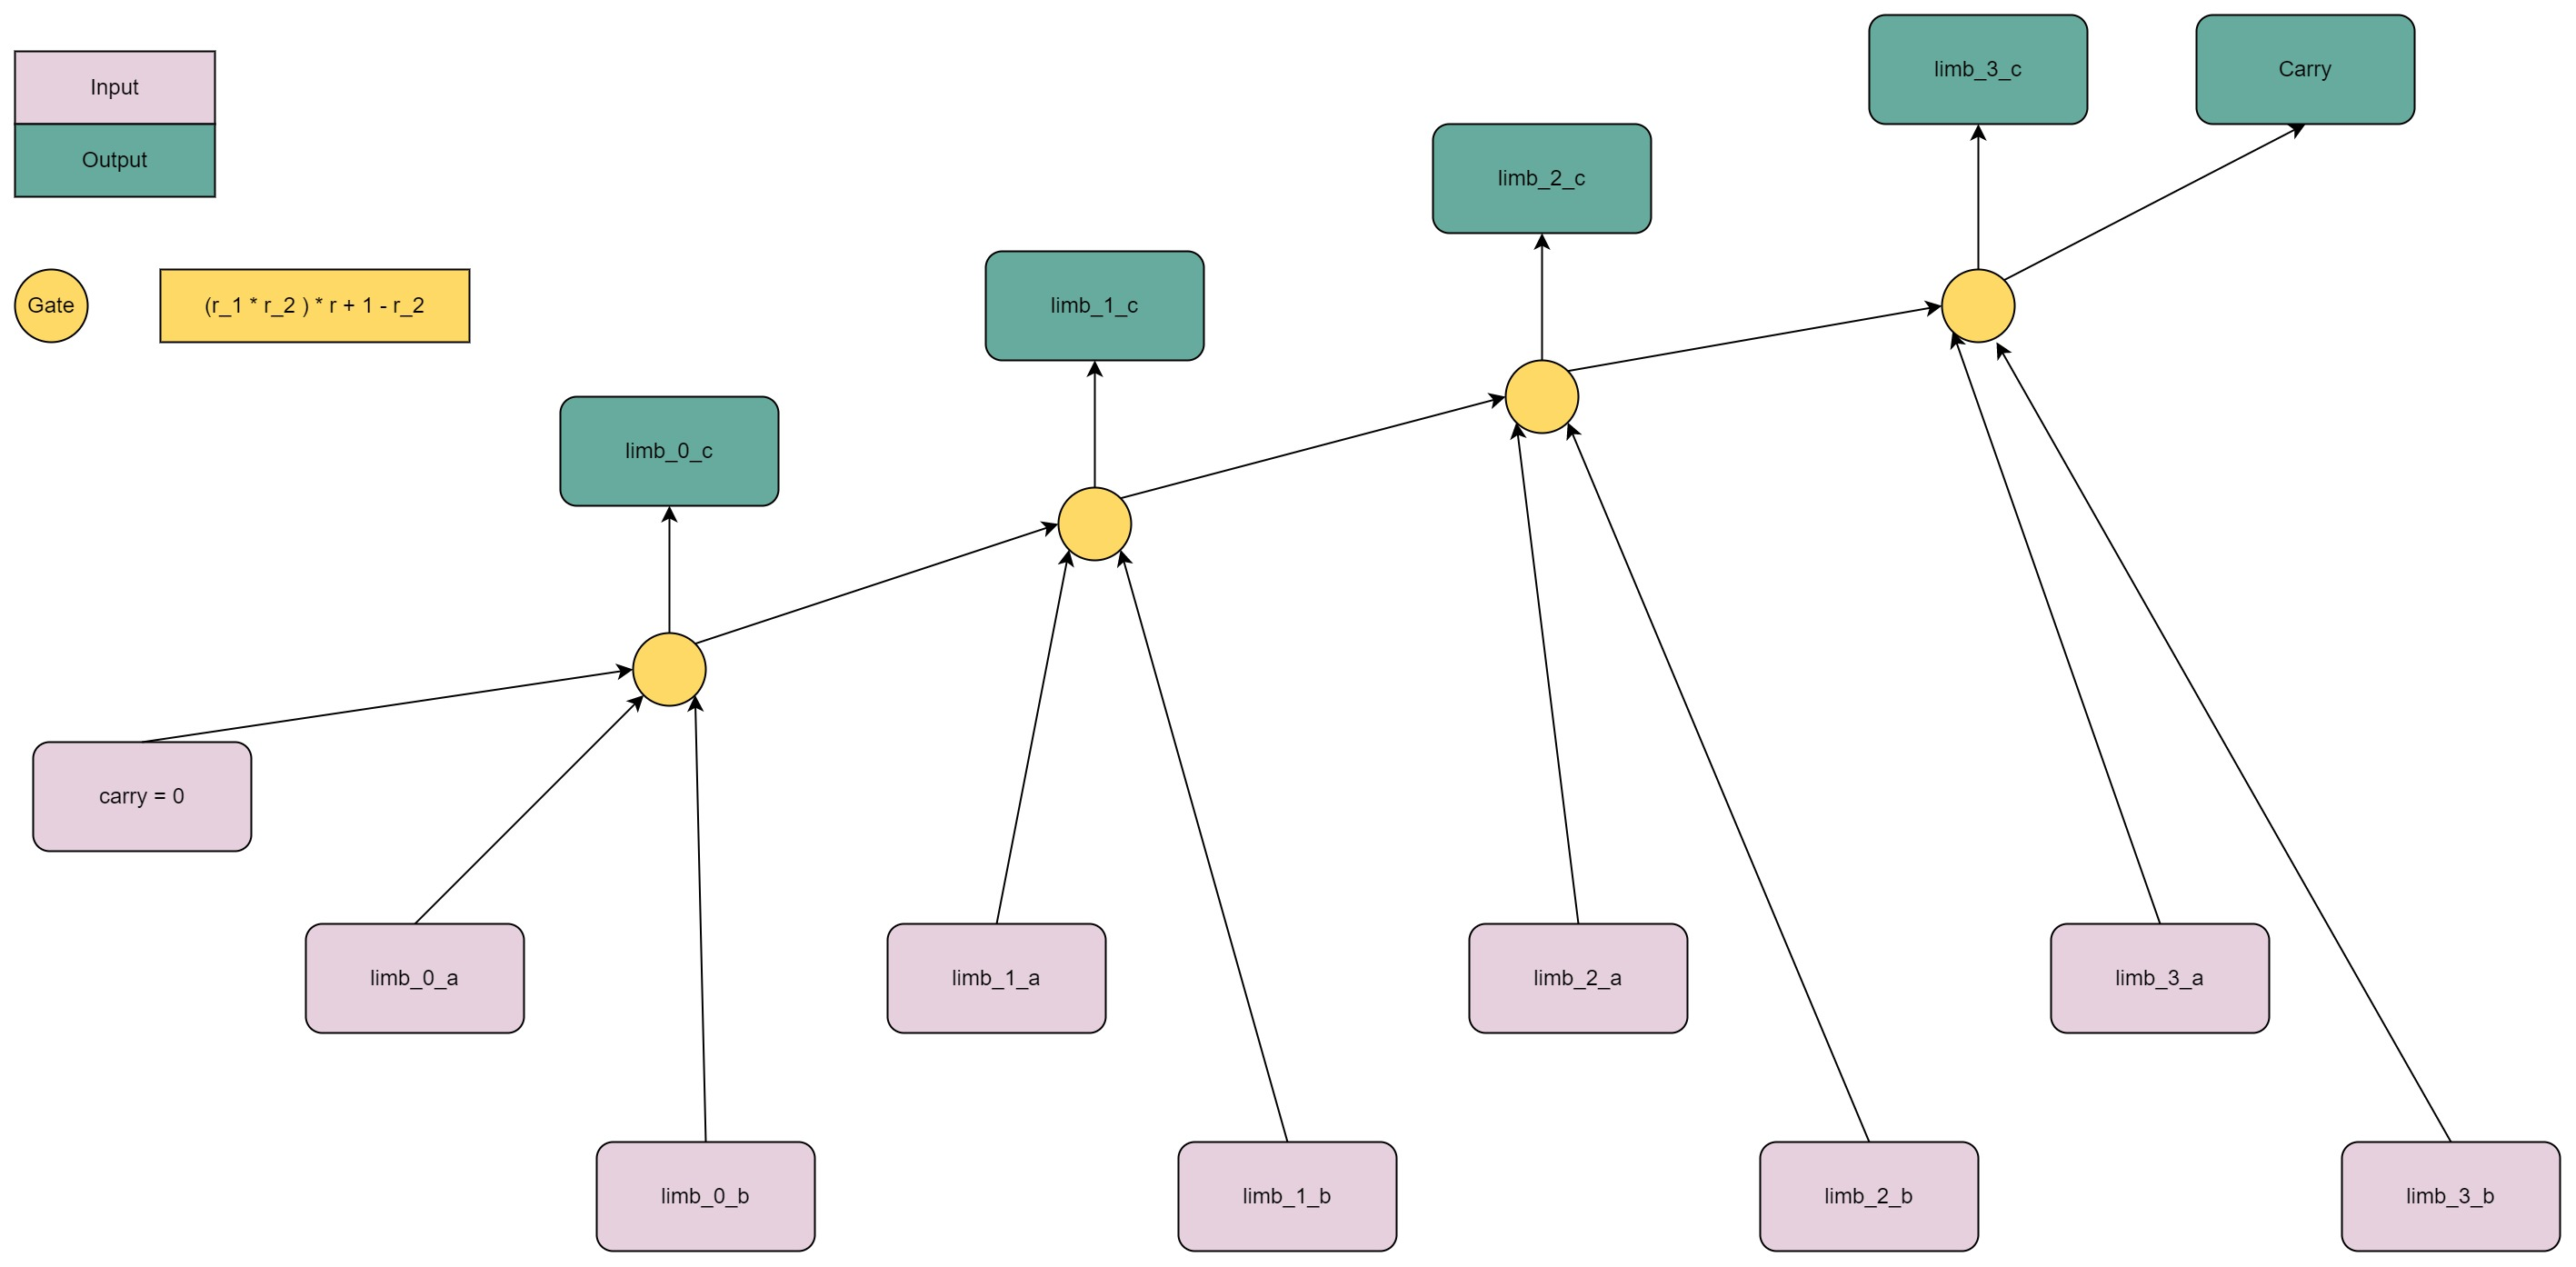
\includegraphics[width=0.8\textwidth]{add_biguint_circuit_layout.jpg}
            \caption{Add_biguint circuit layout}
            \label{fig:add_biguint_circuit_layout}
        \end{figure}

    \item trace layout
        \begin{figure}[!ht]
            \centering
            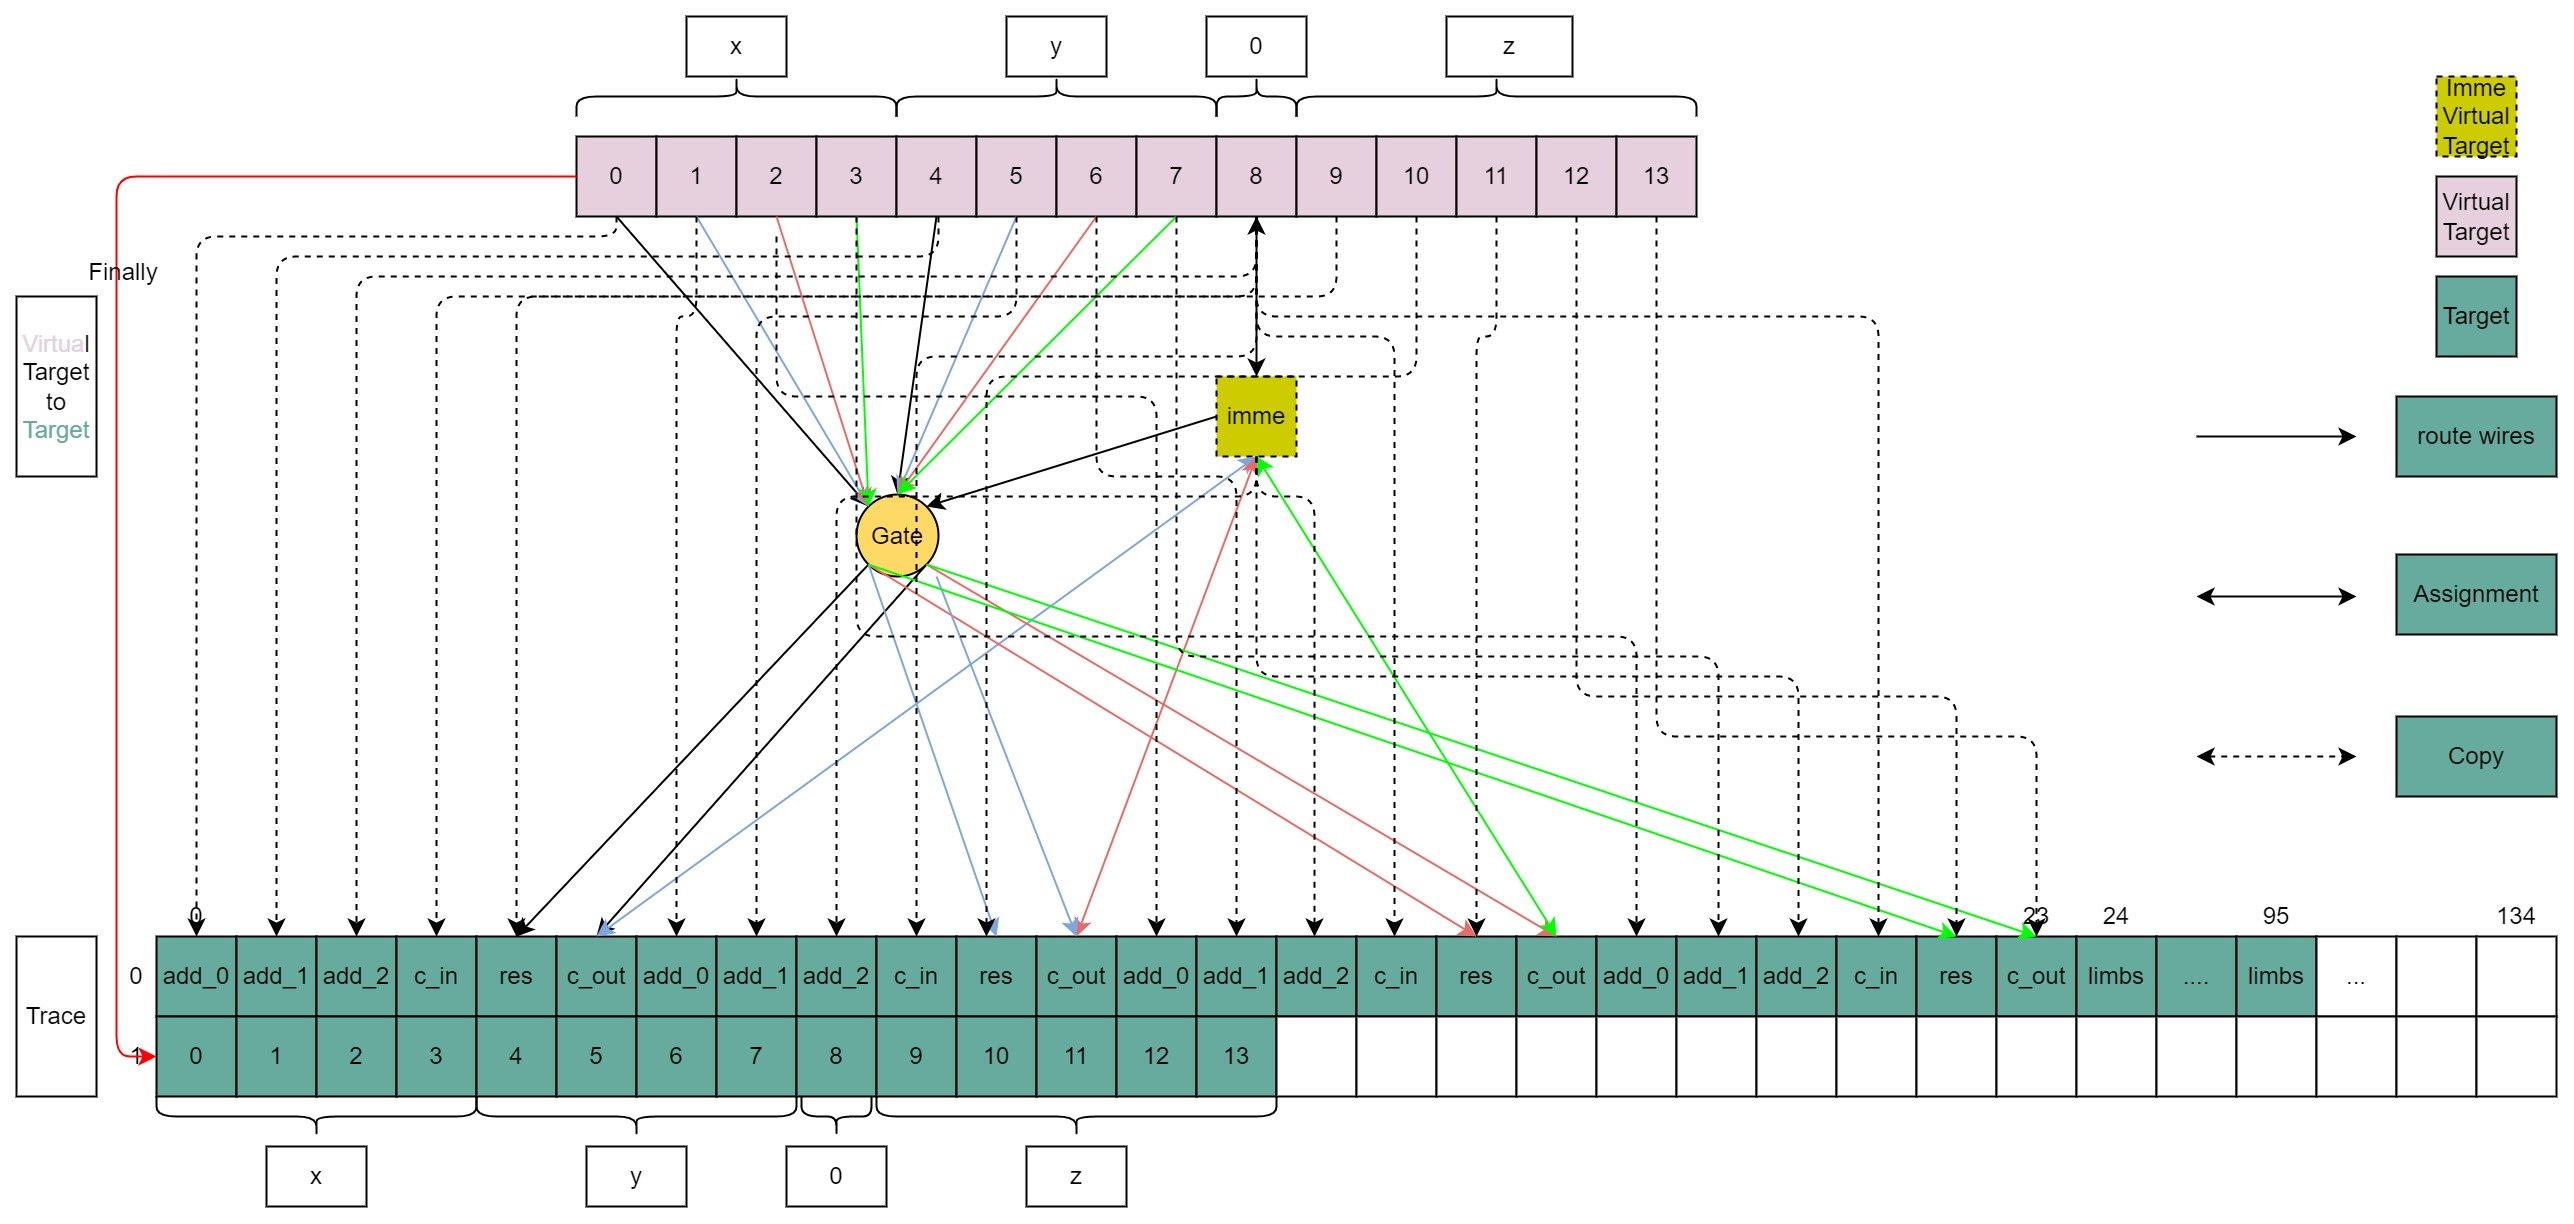
\includegraphics[width=0.8\textwidth]{add_biguint_trace_layout.jpg}
            \caption{Add_biguint trace layout}
            \label{fig:add_biguint_trace_layout}
        \end{figure}
    
    \item constraints-info and costs
        \begin{itemize}
            \item constraints_num: 5 * (3 + 32 / 2 + 4 / 2) = 105
            \item copy_constraints: 4 * 5 + 6 = 26
            \item max_degree: 4
            \item wires_num: 5 * (6 + 16 + 2) = 120
        \end{itemize}

    \item questions
        \begin{itemize}
            \item why not make rangecheck constraint for inputs?
            \item why not make copy constraint between cur_c_in and last_c_out?
        \end{itemize}

\end{enumerate}